\documentclass{standalone}
\usepackage{tikz}
\usetikzlibrary{patterns, positioning}
\usepackage[sfdefault]{ClearSans} %% option 'sfdefault' activates Clear Sans as the default text font
\usepackage[T1]{fontenc}

\begin{document}
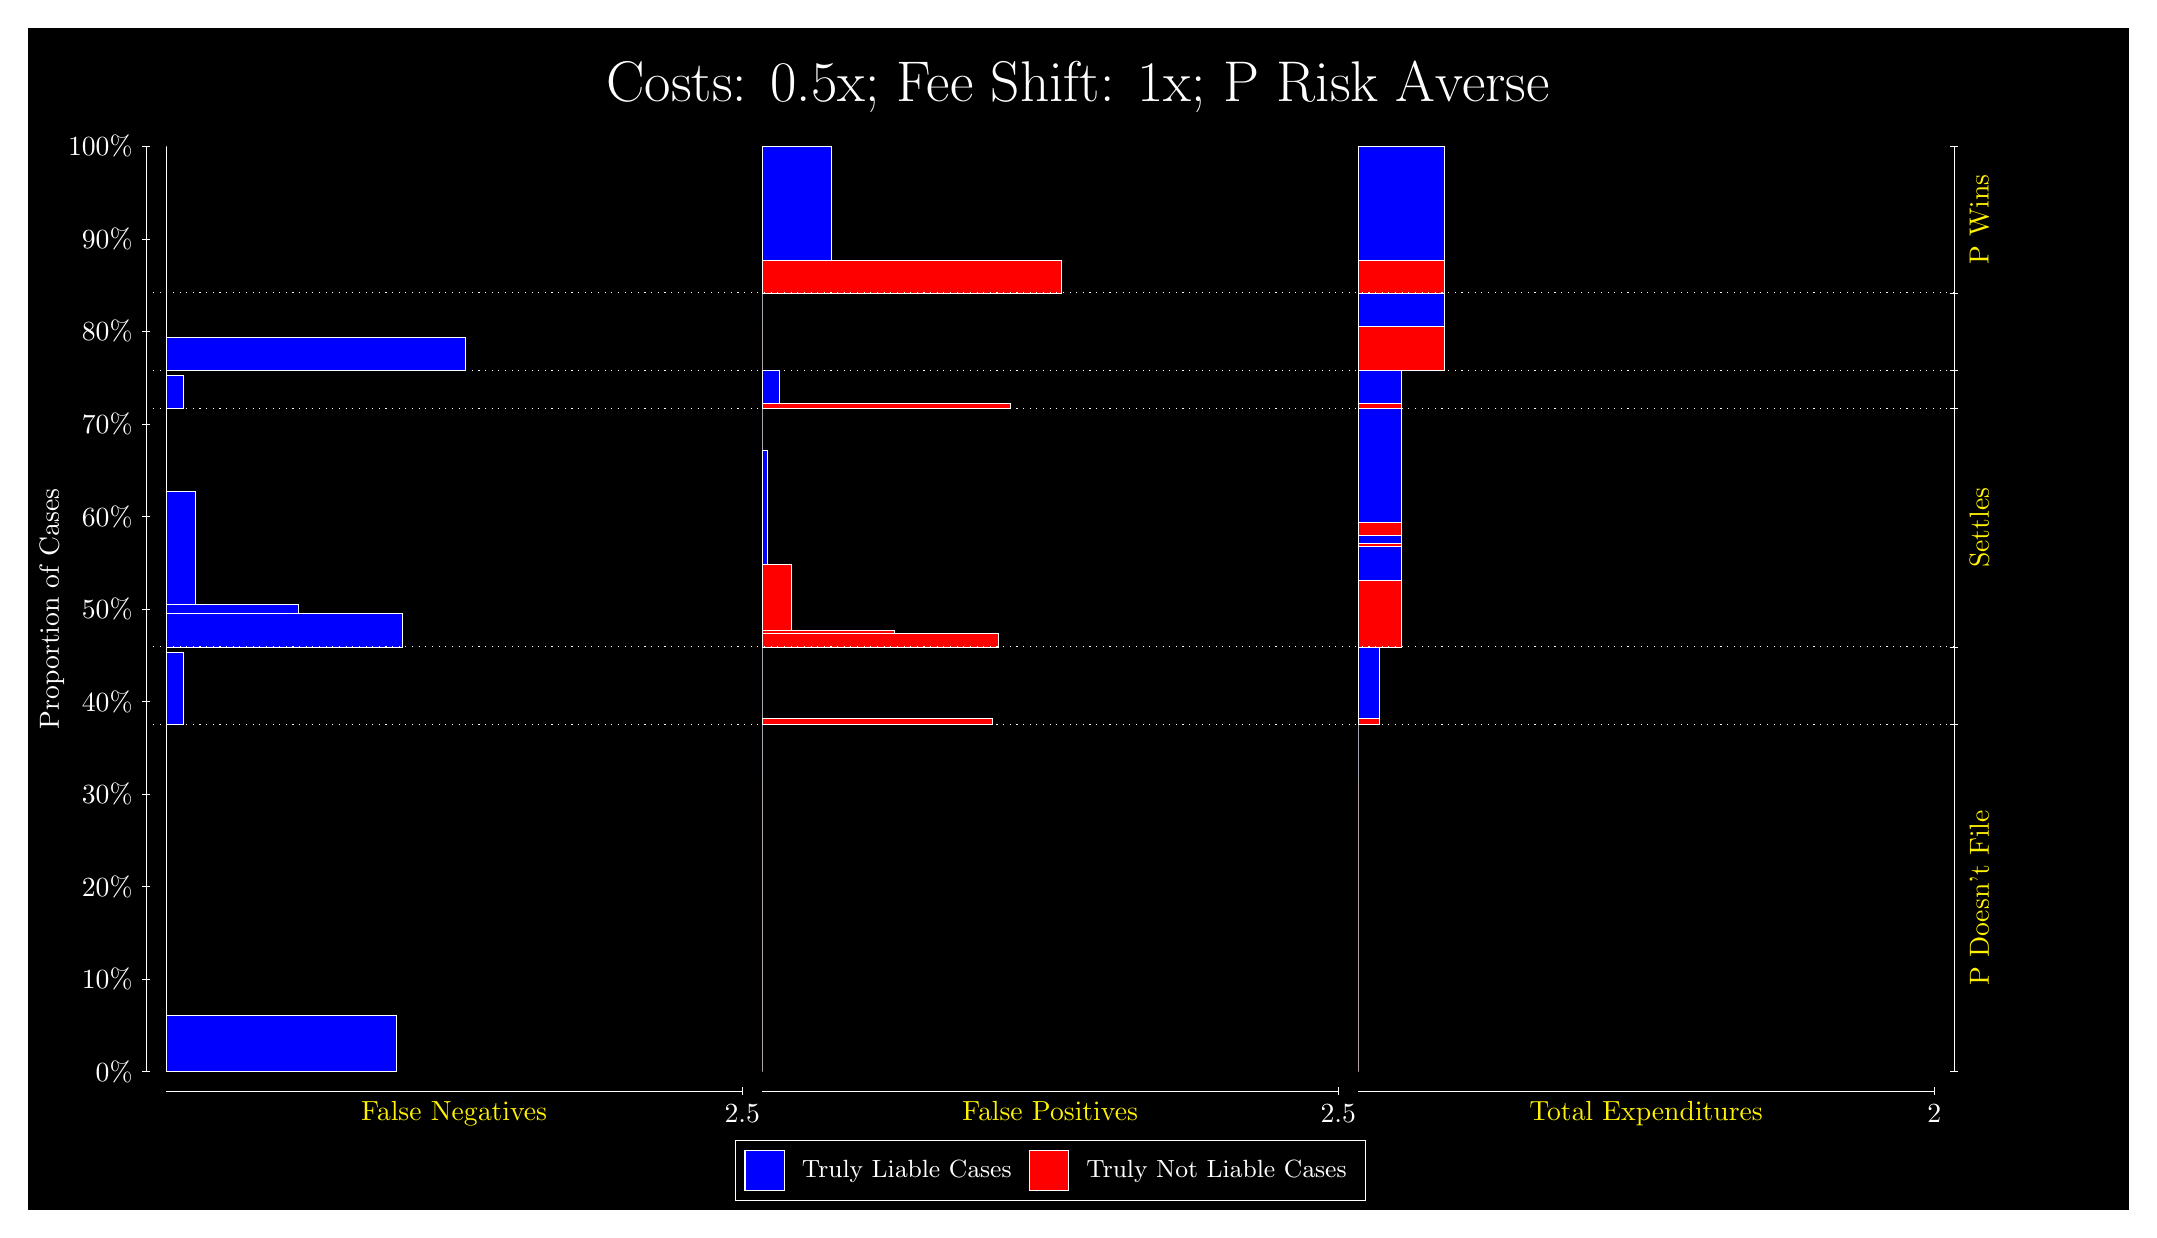
\begin{tikzpicture}
\draw[fill=black] (0,0) rectangle (26.667,15);
\draw[text=white] (0,13.5) rectangle (26.667,15) node[midway] {\huge Costs: 0.5x; Fee Shift: 1x; P Risk Averse};
\draw[white, very thin] (1.5,1.75) -- (1.5,13.5);
\node[rotate=90, text=white, anchor=center] at (0.3, 7.625) {Proportion of Cases};
\draw[white, very thin] (1.45,1.75) -- (1.55,1.75);
\node[text=white, anchor=east] at (1.45, 1.75) {0\%};
\draw[white, very thin] (1.45,2.925) -- (1.55,2.925);
\node[text=white, anchor=east] at (1.45, 2.925) {10\%};
\draw[white, very thin] (1.45,4.1) -- (1.55,4.1);
\node[text=white, anchor=east] at (1.45, 4.1) {20\%};
\draw[white, very thin] (1.45,5.275) -- (1.55,5.275);
\node[text=white, anchor=east] at (1.45, 5.275) {30\%};
\draw[white, very thin] (1.45,6.45) -- (1.55,6.45);
\node[text=white, anchor=east] at (1.45, 6.45) {40\%};
\draw[white, very thin] (1.45,7.625) -- (1.55,7.625);
\node[text=white, anchor=east] at (1.45, 7.625) {50\%};
\draw[white, very thin] (1.45,8.8) -- (1.55,8.8);
\node[text=white, anchor=east] at (1.45, 8.8) {60\%};
\draw[white, very thin] (1.45,9.975) -- (1.55,9.975);
\node[text=white, anchor=east] at (1.45, 9.975) {70\%};
\draw[white, very thin] (1.45,11.15) -- (1.55,11.15);
\node[text=white, anchor=east] at (1.45, 11.15) {80\%};
\draw[white, very thin] (1.45,12.325) -- (1.55,12.325);
\node[text=white, anchor=east] at (1.45, 12.325) {90\%};
\draw[white, very thin] (1.45,13.5) -- (1.55,13.5);
\node[text=white, anchor=east] at (1.45, 13.5) {100\%};

\draw[white, very thin] (24.457,1.75) -- (24.457,13.5);
\draw[white, very thin] (24.407,1.75) -- (24.507,1.75);
\node[anchor=west] at (24.407, 1.75) {};
\draw[white, very thin] (24.407,6.159) -- (24.507,6.159);
\node[anchor=west] at (24.407, 6.159) {};
\draw[white, very thin] (24.407,7.1434) -- (24.507,7.1434);
\node[anchor=west] at (24.407, 7.1434) {};
\draw[white, very thin] (24.407,10.169) -- (24.507,10.169);
\node[anchor=west] at (24.407, 10.169) {};
\draw[white, very thin] (24.407,10.65) -- (24.507,10.65);
\node[anchor=west] at (24.407, 10.65) {};
\draw[white, very thin] (24.407,11.639) -- (24.507,11.639);
\node[anchor=west] at (24.407, 11.639) {};
\draw[white, very thin] (24.407,13.5) -- (24.507,13.5);
\node[anchor=west] at (24.407, 13.5) {};

\draw[white, very thin, fill=blue] (1.75,1.75) rectangle (4.6775,2.4595);
\draw[white, very thin, fill=red] (1.75,2.4595) rectangle (1.75,6.159);
\draw[white, very thin, fill=blue] (1.75,6.159) rectangle (1.9696,7.0696);
\draw[white, very thin, fill=red] (1.75,7.0696) rectangle (1.75,7.1434);
\draw[white, very thin, fill=blue] (1.75,7.1434) rectangle (4.7507,7.5757);
\draw[white, very thin, fill=blue] (1.75,7.5757) rectangle (3.4333,7.678);
\draw[white, very thin, fill=blue] (1.75,7.678) rectangle (2.1159,9.1179);
\draw[white, very thin, fill=red] (1.75,9.1179) rectangle (1.75,10.169);
\draw[white, very thin, fill=blue] (1.75,10.169) rectangle (1.9696,10.587);
\draw[white, very thin, fill=red] (1.75,10.587) rectangle (1.75,10.65);
\draw[white, very thin, fill=blue] (1.75,10.65) rectangle (5.5558,11.069);
\draw[white, very thin, fill=red] (1.75,11.069) rectangle (1.75,11.639);
\draw[white, very thin, fill=red] (1.75,11.639) rectangle (1.75,12.056);
\draw[white, very thin, fill=blue] (1.75,12.056) rectangle (1.75,13.5);
\draw[white, very thin, fill=red] (9.3189,1.75) rectangle (9.3189,5.4495);
\draw[white, very thin, fill=blue] (9.3189,5.4495) rectangle (9.3189,6.159);
\draw[white, very thin, fill=red] (9.3189,6.159) rectangle (12.246,6.2328);
\draw[white, very thin, fill=blue] (9.3189,6.2328) rectangle (9.3189,7.1434);
\draw[white, very thin, fill=red] (9.3189,7.1434) rectangle (12.32,7.3137);
\draw[white, very thin, fill=red] (9.3189,7.3137) rectangle (11.002,7.3525);
\draw[white, very thin, fill=red] (9.3189,7.3525) rectangle (9.6848,8.1947);
\draw[white, very thin, fill=blue] (9.3189,8.1947) rectangle (9.3921,9.6346);
\draw[white, very thin, fill=blue] (9.3189,9.6346) rectangle (9.3189,10.169);
\draw[white, very thin, fill=red] (9.3189,10.169) rectangle (12.466,10.232);
\draw[white, very thin, fill=blue] (9.3189,10.232) rectangle (9.5384,10.65);
\draw[white, very thin, fill=red] (9.3189,10.65) rectangle (9.3189,11.22);
\draw[white, very thin, fill=blue] (9.3189,11.22) rectangle (9.3189,11.639);
\draw[white, very thin, fill=red] (9.3189,11.639) rectangle (13.125,12.056);
\draw[white, very thin, fill=blue] (9.3189,12.056) rectangle (10.197,13.5);
\draw[white, very thin, fill=red] (16.888,1.75) rectangle (16.888,5.4495);
\draw[white, very thin, fill=blue] (16.888,5.4495) rectangle (16.888,6.159);
\draw[white, very thin, fill=red] (16.888,6.159) rectangle (17.162,6.2328);
\draw[white, very thin, fill=blue] (16.888,6.2328) rectangle (17.162,7.1434);
\draw[white, very thin, fill=red] (16.888,7.1434) rectangle (17.437,7.9856);
\draw[white, very thin, fill=blue] (16.888,7.9856) rectangle (17.437,8.4179);
\draw[white, very thin, fill=red] (16.888,8.4179) rectangle (17.437,8.4567);
\draw[white, very thin, fill=blue] (16.888,8.4567) rectangle (17.437,8.559);
\draw[white, very thin, fill=red] (16.888,8.559) rectangle (17.437,8.7293);
\draw[white, very thin, fill=blue] (16.888,8.7293) rectangle (17.437,10.169);
\draw[white, very thin, fill=red] (16.888,10.169) rectangle (17.437,10.232);
\draw[white, very thin, fill=blue] (16.888,10.232) rectangle (17.437,10.65);
\draw[white, very thin, fill=red] (16.888,10.65) rectangle (17.986,11.22);
\draw[white, very thin, fill=blue] (16.888,11.22) rectangle (17.986,11.639);
\draw[white, very thin, fill=red] (16.888,11.639) rectangle (17.986,12.056);
\draw[white, very thin, fill=blue] (16.888,12.056) rectangle (17.986,13.5);
\draw[white, dotted] (1.5,6.159) -- (24.457,6.159);
\draw[white, dotted] (1.5,7.1434) -- (24.457,7.1434);
\draw[white, dotted] (1.5,10.169) -- (24.457,10.169);
\draw[white, dotted] (1.5,10.65) -- (24.457,10.65);
\draw[white, dotted] (1.5,11.639) -- (24.457,11.639);
\draw[white, very thin] (1.75,1.5) -- (9.0689,1.5);
\node[text=yellow, anchor=north] at (5.4094, 1.5) {False Negatives};
\draw[white, very thin] (9.0689,1.45) -- (9.0689,1.55);
\node[text=white, anchor=north] at (9.0689, 1.45) {2.5};

\draw[white, very thin] (9.3189,1.5) -- (16.638,1.5);
\node[text=yellow, anchor=north] at (12.978, 1.5) {False Positives};
\draw[white, very thin] (16.638,1.45) -- (16.638,1.55);
\node[text=white, anchor=north] at (16.638, 1.45) {2.5};

\draw[white, very thin] (16.888,1.5) -- (24.207,1.5);
\node[text=yellow, anchor=north] at (20.547, 1.5) {Total Expenditures};
\draw[white, very thin] (24.207,1.45) -- (24.207,1.55);
\node[text=white, anchor=north] at (24.207, 1.45) {2};

\node[text=yellow, centered, rotate=90] at (24.777, 3.9545) {P Doesn't File};

\node[text=yellow, centered, rotate=90] at (24.777, 8.6563) {Settles};


\node[text=yellow, centered, rotate=90] at (24.777, 12.569) {P Wins};

\draw (12.978300999999998,1.5) node[draw=none] (baseCoordinate) {};
\begin{scope}[align=center]
        \matrix[scale=0.5, draw=white, below=0.5cm of baseCoordinate, nodes={draw}, column sep=0.1cm]{
            \node[rectangle, draw, minimum width=0.5cm, minimum height=0.5cm, fill=blue] {}; &
            \node[draw=none, font=\small, text=white] (B) {Truly Liable Cases}; &
            \node[rectangle, draw, minimum width=0.5cm, minimum height=0.5cm, fill=red] {}; &
            \node[draw=none, font=\small, text=white] (B) {Truly Not Liable Cases}; \\
            };
\end{scope}

\end{tikzpicture}
\end{document}